%********VORAUSSETZUNGEN & GRUNDLAGEN*********
\section{Fundamentals}
\label{sec:fundamentals}

\subsection{Laser Principles}
    % Explain the basic principles of lasers, including stimulated emission, population inversion, and coherence.
    % Discuss their importance in scientific and technological applications.
    
    \subsubsection{Stimulated emission}
    Stimulated emission occurs when a photon of a particular frequency interacts with an already excited atomic electron or another excited molecular state, prompting it to transition to a lower energy level.
   
    
    \begin{wrapfigure}[13]{r}[0cm]{0.3\textwidth}
        \centering
        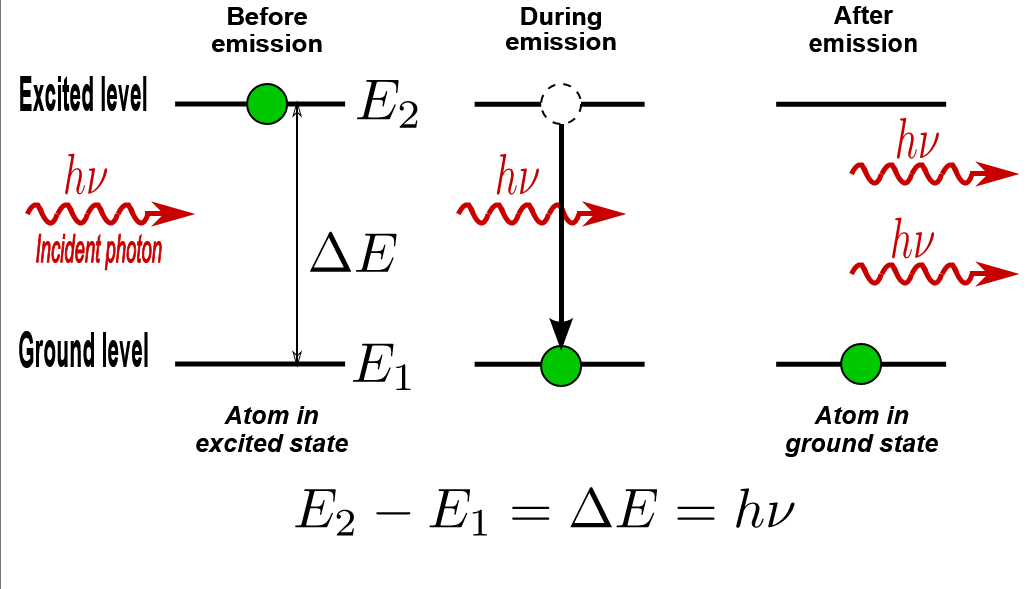
\includegraphics[width=0.3\textwidth]{Stim_Emission.png}
        
        \caption[width = 0.1\textwidth]{ Stimulated Emission  \cite{Laser_cav} }
        \label{fig:energy_diagram}
    \end{wrapfigure}
    \noindent In response to a external electromagnetic field at a frequency associated with a transition between two stationary states, the likelyhood of an electron entering this transition state is greatly increased.
    This increases the probability of transition beyond that of spontanious emission. 
    By means of population inversion $N_2$/$N_1$ > 1, where $N_2$ is the population in the excited state and $N_1$ is the population in the ground state, the function of the laser is optimized.
    In other words, the population of the excited state must exceed that of the ground state.
    This allows for the production of a continuously increasing number of photons, establishing a higher output power for the laser medium.
    Understanding the interplay between absorption, stimulated emission, and population inversion is crucial for the design and operation of laser systems.
    By harnessing stimulated emission and achieving population inversion, lasers can produce a coherent light source. \cite{Laser_cav}
    %\monofig{width = 0.5\textwidth}{Stim_Emission.png}{ Stimulated Emission  \cite{Laser_cav} }{fig:energy_diagram}

\subsubsection{Pulsed Lasers (Mode Locking)}
    % Describe pulsed lasers, their advantages, and limitations.
    % Discuss the concept of time-bandwidth limit and its relevance.
    In order to generate ultra-short pulses of light in the range of picoseconds or femtoseconds, an optics technique called Mode Locking is used.
If the length of the laser's optical cavity is a multiple of the laser's fundamental frequency, standing waves or modes arise.
By fixing the phase relationship between the longetudinal modes, constructive interference between the standing waves is achieved, which produces synchronized pulses.
This method, known as mode locking, alters the behavior of the laser's modes, causing them to periodically constructively interfere and emit intense bursts of light.
The pulse duration is determined by the number of locked modes and their frequency separation, which is governed by the laser's spectral width.
    
\subsection{Second Harmonic Generation (SHG)}
    % Introduce SHG as a nonlinear optical process.
    % Explain how crystals generate light at twice the input frequency.
    % Discuss the importance of phase matching.
    %Second-harmonic generation (SHG), or frequency doubling, is a fundamental nonlinear optical process where two photons with the same frequency interact in a nonlinear material, combining to generate a new photon with double the energy.
    %This results in a photon with twice the frequency and half the wavelength of the initial photons,
    Second-harmonic generation (SHG) is a nonliniar optical process ,which is characterized by the second-order nonliniar susceptibility $\chi^{2}$ of a optical medium.
    In systems in which $\chi^{2}$ is non vanishing, two photons with the same frequency interact to form a photon with double the frequency and half the wavelength.
    To archieve a high conversion efficiency the phase velocities of the incident wave and SH wave must be equal. \cite{demtroder2014laser}
     
    \begin{wrapfigure}[7]{r}[0cm]{0.4\textwidth}
        \centering
        \vspace{-\normalbaselineskip}
        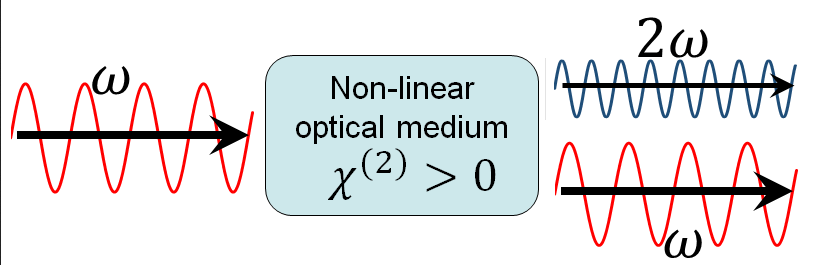
\includegraphics[width=0.4\textwidth]{shg_schem.png}
        \vspace{-10pt}
        \caption{Second harmonic generation \cite{shg}  }
        
        \label{fig:shg:basic}
    \end{wrapfigure}
    In negative birefringent uniaxial crystals, this is done by rotating the crystal in a certain direction where the extraordinary refractive index $n(2\omega)$ of the SH wave is equal to the ordinary refractive index $n(\omega)$ of the fundamental wavelength.
    The polarization direction of the SH wave is therefore orthogonal to that of the fundamental wave.
    For positive birefringent uniaxial crystals, it is switched, which means that the SH wave travels as an ordinary wave outside the medium.
    %conserving excitation coherence. SHG is utilized extensively, particularly in doubling laser frequencies, and is governed by the second-order nonlinear susceptibility of the medium. 
    %While SHG is typically prohibited in media with inversion symmetry, exceptions exist, such as in non-centrosymmetric crystals. 
    %Achieving efficient SHG often requires intense pulsed laser beams passing through large crystals with precise alignment for phase matching.

\subsection{Iodine Absorption \& Concentration}
    % Cover the absorption properties of iodine, including rotation, vibration, and temperature dependence.
    % Explain natural linewidth and temperature broadening effects.

Molecular iodine, which in the experiment described in the present document is examined in the gas phase as a diatomic molecule, exhibits absorption properties in the visible spectral range. These absorption properties, on one hand, arise due to the vibrational and rotational structure and the corresponding degrees of freedom of such molecules. On the other hand, electronic state transitions from ground states to excited states enable further absorption of specific wavelengths in the visible range \cite{demtroder2014laser}.

The absorption lines apparent in the absorption spectrum are expected to be slim and narrowly centered around the characteristic wavelengths corresponding to valid state transitions. There are a number of effects that lead to the broadening of these spectral lines, most importantly the intrinsic natural broadening arising from the finite lifetime of excited states. A second important effect is called temperature broadening, which results from the thermal motion of particles due to the Doppler effects. The latter effect only becomes apparent at high temperatures of the sample however \cite{demtroder2014laser}.

The decadic absorbance $A$ is described by
\begin{equation}
    \label{eq:fundamentals:absorbance}
    A = \log_{10}\left(\frac{I_0}{I_t}\right) ,
\end{equation}
where $I_0$ is the measured laser intensity without iodine and $I_t$ is the intensity transmitted by the iodine \cite{demtroder2014laser}. For small molar concentrations $c$, the Lambert-Beer law relates the absorbance $A$ to the effective interaction length $l$ of the laser beam with the iodine and the molecular absorption coefficient $\varepsilon$ as follows \cite{attenuation}.
\begin{equation}
    \label{eq:fundamentals:beer}
    A = l \cdot c \cdot \varepsilon
\end{equation}

The absorption cross-section $\sigma$ of iodine, which is a measure for the probability of an absorption process, commonly denoted in units of \si{\cm\squared\per\molecule} and available in scientific literature such as \cite{Iodine}, can be used to obtain the molecular absorption coefficient $\varepsilon$ via the relation
\begin{equation}
    \label{eq:fundamentals:absorptivity}
    \sigma = \frac{\ln(10) \cdot 10^3}{N_A} \cdot \varepsilon ,
\end{equation}
where $N_A$ is the Avogadro Constant \cite{attenuation}. The molecular absorption coefficient is commonly specified in units of \si{\liter\per\mol\per\cm} and - contrary to the absorbance $A$ - uses $e$ as logarithmic base, explaining the need for the term $ln(10) \cdot 10^3$ in Equation \ref{eq:fundamentals:absorptivity} due to base and unit conversion.


\subsection{Grating Spectrometer}
% Briefly mention grating spectrometers and their role in analyzing laser spectra.
% Explain how diffraction gratings disperse light for spectral measurements.

Spectrometers in general are optical instruments that create images which are laterally separated for different wavelengths $\lambda$ of the incident radiation. In the case of a grating spectrometer, as opposed to spectral dispersion used in a prism spectrometer, the lateral dispersion is due to diffraction plane or concave reflection gratings \cite{demtroder2014laser}.
\begin{wrapfigure}[14]{r}[0cm]{0.4\textwidth}
    \centering
    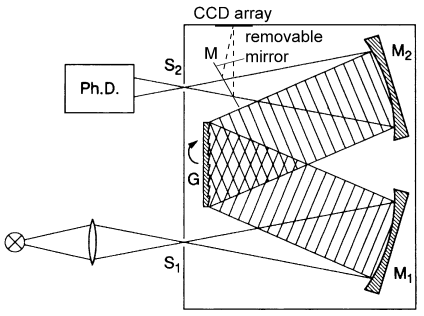
\includegraphics[width=0.3\textwidth]{graphics/spectrometer.png}
    
    \caption[width = 0.1\textwidth]{Schematic structure of a grating spectrometer \cite{demtroder2014laser}.}
    \label{fig:fundamentals:spectrometer}
\end{wrapfigure}
In a grating spectrometer as shown in Figure \ref{fig:fundamentals:spectrometer}, the light source illuminates the entrance slit $S_1$, which is in the focal plane of a spherical mirror $M_1$. The collimated, parallel light is reflected by $M_1$ onto a reflection grating consisting of many straight grooves parallel to the entrance slit. Highly reflective metal or dielectric coating on the surface of the grating is used to reflect the light towards a second spherical mirror $M_2$,which in turn focuses it onto the exit slit $S_2$ or onto a photographic plate in the focal plane of $M_2$ \cite{demtroder2014laser}.

%\begin{figure}[H]
%    \centering
%    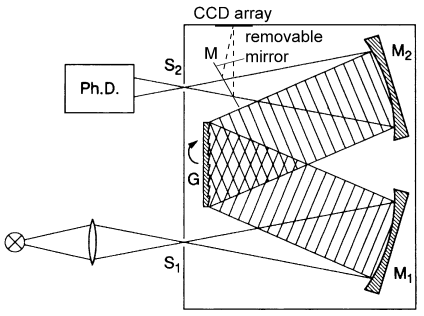
\includegraphics[width=0.45\textwidth]{graphics/spectrometer.png}
%    \caption{Schematic structure of a grating spectrometer \cite{demtroder2014laser}.}
%    \label{fig:fundamentals:spectrometer}
%\end{figure}

\noindent Considering the coherently illuminated grooves on the grating as individual sources of radiation, each of them diffracting the incident light into a larger range around the direction nof geometrical reflection, the resulting outgoing intensity is subject to destructive and constructive interference, where for the latter the grating equation is
\begin{equation}
    \label{eq:fundamentals:grating}
    2 d \cdot \sin(\alpha) = m \lambda ,
\end{equation}
where $d$ is the width of each groove and $\alpha$ is the angle of the $m$-th order maximum at incident wavelength $\lambda$ \cite{demtroder2014laser}. From Equation \ref{eq:fundamentals:grating} follows the spectral resolving power as
\begin{equation}
    \label{eq:fundamentals:resolving}
    R = \frac{\lambda}{\Delta \lambda} = m N ,
\end{equation}
for diffraction order $m$ with the total number $N$ of illuminated grooves \cite{demtroder2014laser}.

While using a prism spectrometer would have the advantage of unambiguous assignment of wavelengths $\lambda$, which is not the case for grating spectrometers due to a diffraction pattern with potentially overlapping orders of diffraction being produced, the former offer only moderate spectral resolution compared to grating spectrometers. Also, since the current experiment involves infrared radiation, for which coated mirrors and gratings exhibit especially high reflectivity, grating spectrometers are preferred over prism spectrometers in such scenarios \cite{demtroder2014laser}.

\newpage